%!TEX root = ../../main.tex
\section{코퍼스와 데이터의 역할}
\label{sec:data-corpus}
\label{sec:data-roles}

원천 코퍼스는 한국(KR) 서버의 랭크 경기 \numMatchesTotal{} 건이다. Match-V5의 \texttt{gameVersion}이 15.14, 15.15, 15.16인 세 패치이며, 공개 번호 25.14--25.16에 대응한다 \cite{lolwiki2026v2514,lolwiki2026v2516}. 수집 경로는 Match-V5이다. 경기 식별자로 경기 문서를 받고, 같은 식별자로 타임라인을 받는다 \cite{riotapi2024matchv5,riotapi2024timeline}. 분석 대상은 각 패치가 적용된 동안 진행된 경기이다. 파일을 받은 시각이 아니다. 어느 패치인지는 \texttt{gameVersion}으로 가른다.

15.14는 학습에, 15.15는 보정과 선정에, 15.16은 평가에 쓴다. 역할은 경기 단위로 배정하므로, 한 경기의 여러 교전이 서로 다른 역할에 들어가지 않는다. 그림 \ref{fig:data-roles}이 이 순서이다. 표 \ref{tab:corpus-census}는 패치별 경기 수와 교전 수이고, 검출된 교전과 유효한 교전을 가르는 규칙은 제 \ref{ch:engagement} 장에 있다. 표의 합계는 코퍼스 전체이고, 주 예측 결과는 15.16의 교전에서만 낸다.

%% figure 객체: fig:data-roles — 패치별 역할. 원본 figures/data_roles.png
\begin{figure}[t]
  \centering
  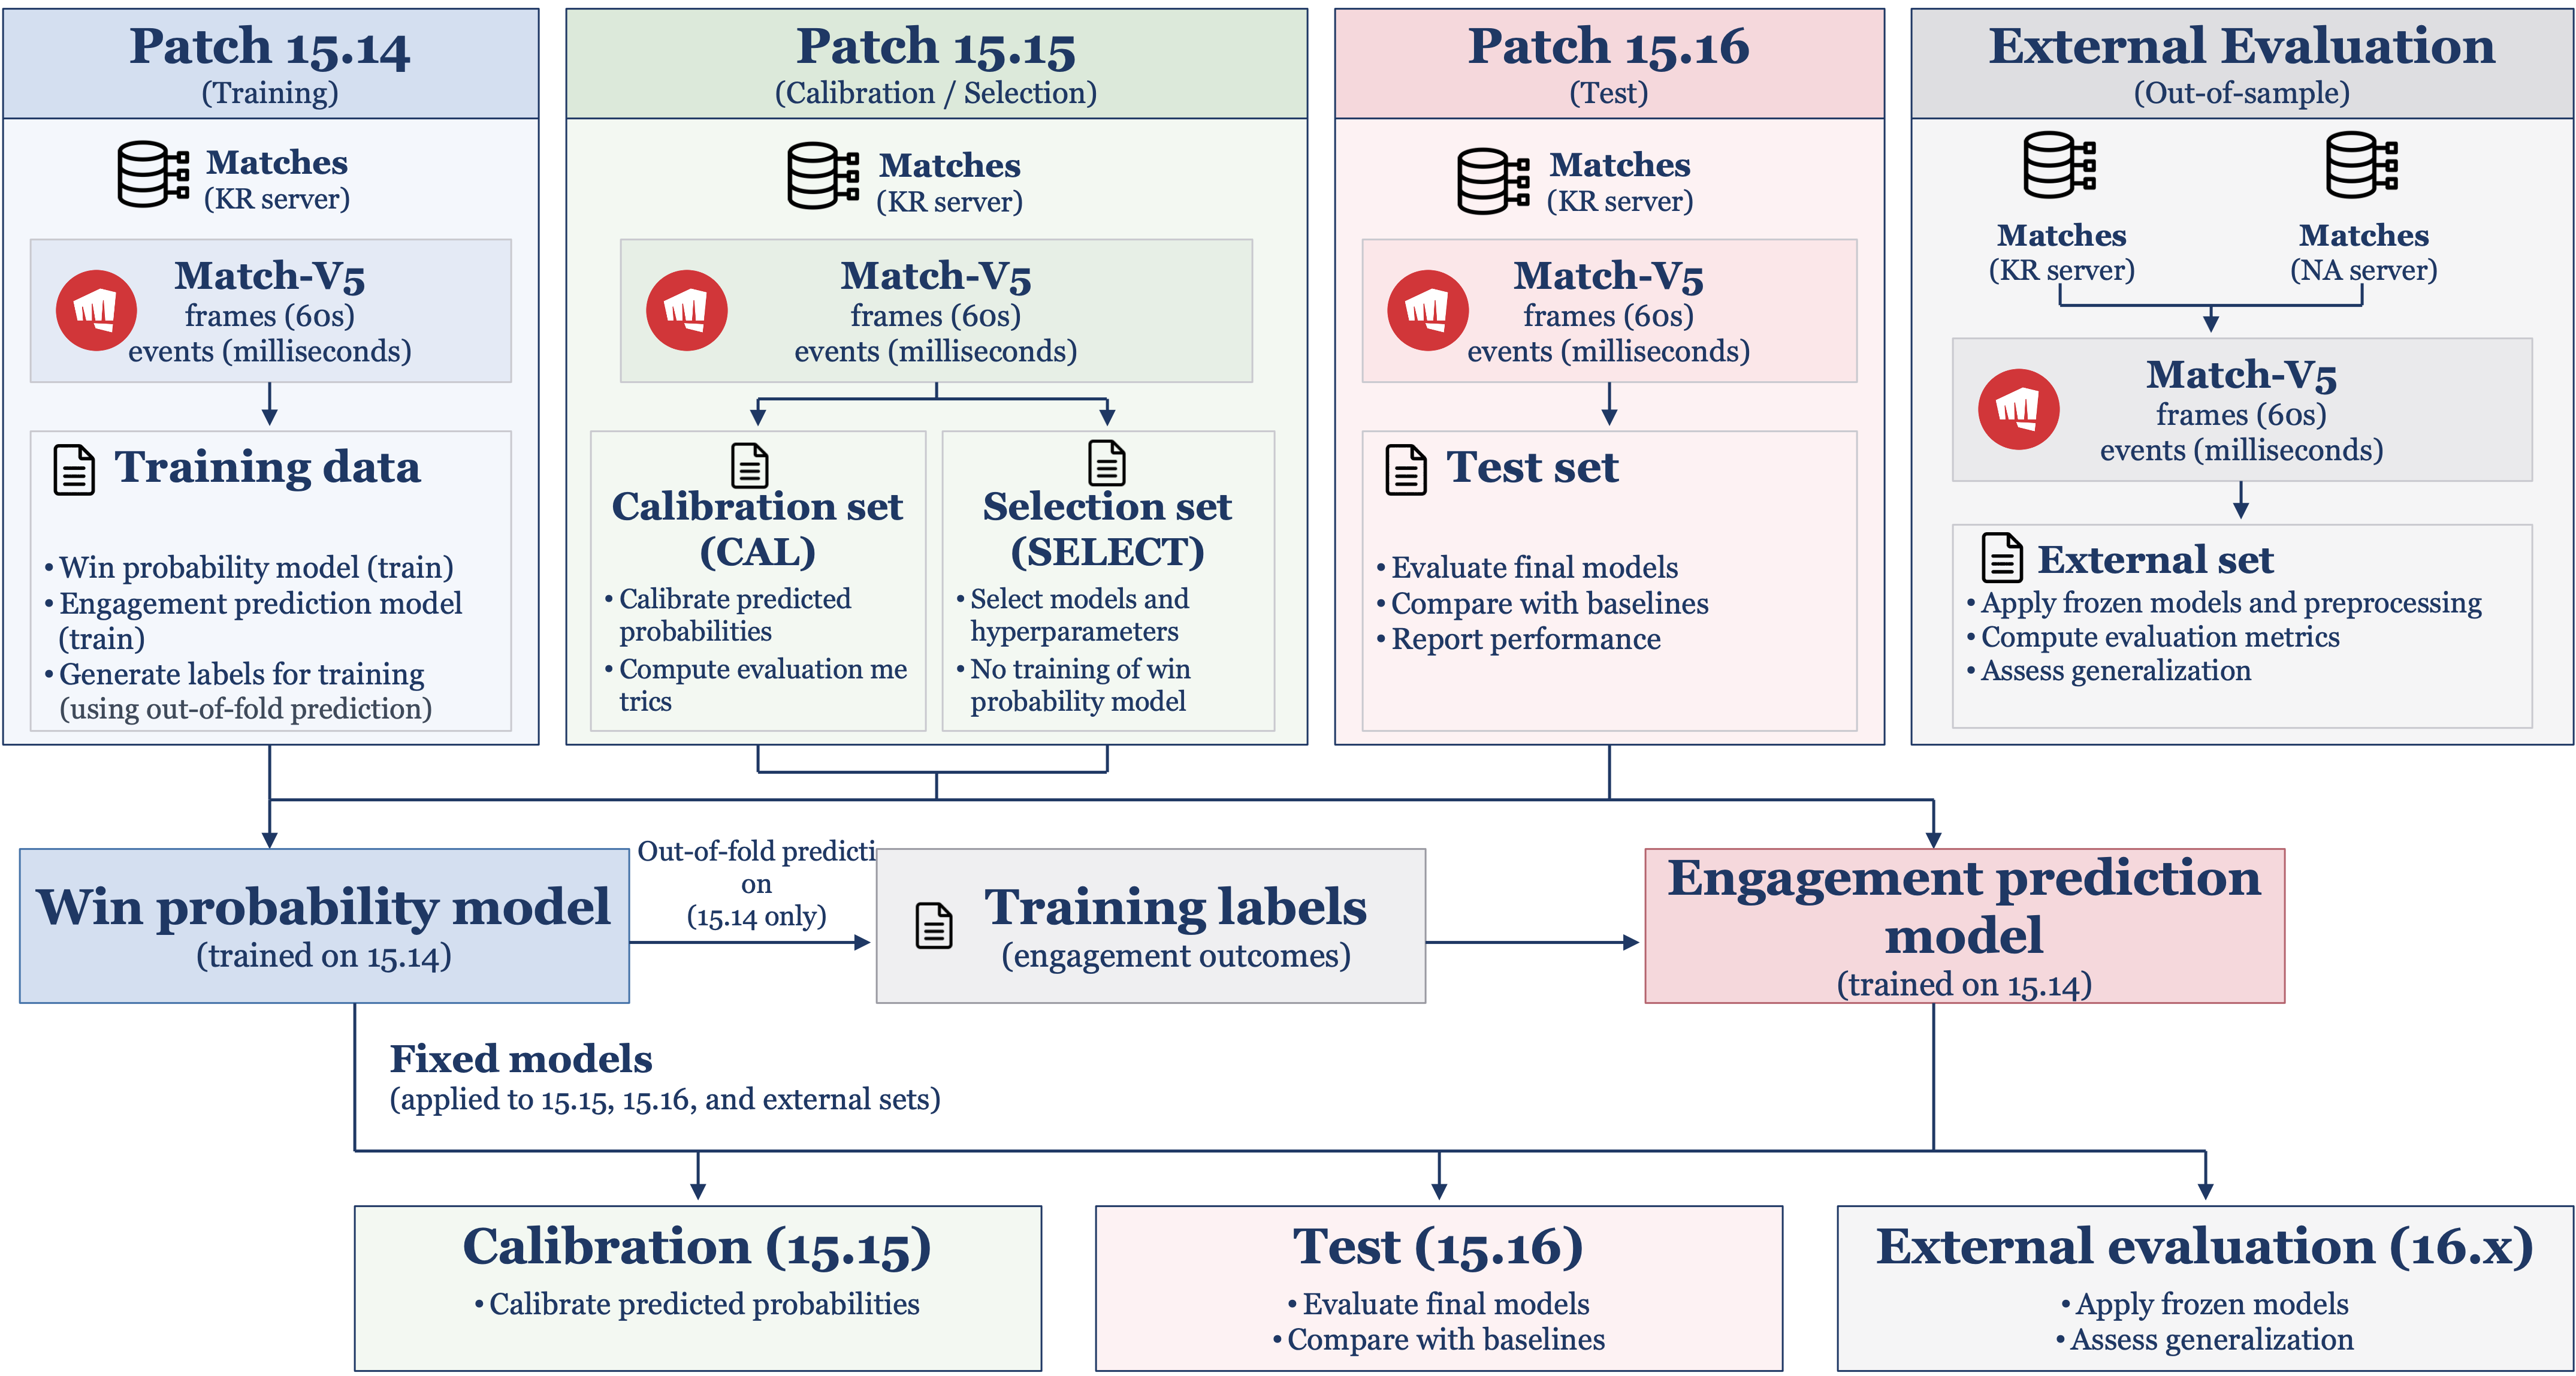
\includegraphics[width=\linewidth]{figures/data_roles.png}
  \caption{패치에 따른 학습, 보정·선정, 평가}
  \label{fig:data-roles}
\end{figure}

%% table 객체: tab:corpus-census — 출처 lineage_20260915/README.md L82–86 (e0ec3d0 manuscript.md L200–208)
\begin{table}[!t]
  \centering
  \caption{패치별 원천 코퍼스}
  \label{tab:corpus-census}
  \small
  \begin{tabular}{@{}llrrrrr@{}}
    \toprule
    역할 & 패치 & 경기 & 검출 교전 & 유효 교전 & T 행 & N 행 \\
    \midrule
    TRAIN & 15.14 & \numMatchesTrain{} & \numEngTrainDet{} & \numEngTrainValid{} & \numTTrain{} & \numNTrain{} \\
    VALIDATION & 15.15 & \numMatchesVal{} & \numEngValDet{} & \numEngValValid{} & \numTVal{} & \numNVal{} \\
    TEST & 15.16 & \numMatchesTest{} & \numEngTestDet{} & \numEngTestValid{} & \numTTest{} & \numNTest{} \\
    \midrule
    합계 & & \numMatchesTotal{} & \numEngDetected{} & \numEngValid{} & \numTPooled{} & \numNPooled{} \\
    \bottomrule
  \end{tabular}
  \tabnote{유효 = 결과 시점 규칙의 유효성 검사를 통과한 교전(제 \ref{sec:eng-endpoint} 절); 세 지평에서 동일하며, 제외된 \numEngInvalid{} 행은 모두 N에 속한다.}
\end{table}


승률 모형은 경기 안의 한 시각마다, 교전의 결과가 오를지를 예측하는 모형은 교전마다 나눈다. 두 모형은 서로 다른 보정·선정 경기를 쓴다. 15.14 교전의 결과는 그 경기를 빼고 다시 만든 승률 모형이 매기고, 그 뒤의 패치에는 15.14로 학습한 뒤 고정한 승률 모형을 쓴다. 표 \ref{tab:roles-evaluator}와 표 \ref{tab:roles-engagement}가 각각의 수이다. 한타와 소규모 교전을 어떻게 고르고 맞추는지는 제 \ref{ch:prediction} 장에 있다.

%% table 객체: tab:roles-evaluator — 출처 A_MLP_expanded_evaluator_meta_20260919.json meta.census; TEST_BAND_LEDGER
\begin{table}[!t]
  \centering
  \caption{승률 평가기 $\Vhat$의 데이터 역할 (시간상태 단위)}
  \label{tab:roles-evaluator}
  \small
  \begin{tabular}{@{}llrrl@{}}
    \toprule
    역할 & 패치 & 시간상태 행 & 경기 & 용도 \\
    \midrule
    TRAIN 적합 & 15.14 & \numVFit{} & --- & 가중치 \\
    TRAIN 정지 & 15.14 & \numVStop{} & --- & 조기 종료 (경기 단위 \holdoutV{}\% 보류, 시드 \bootSeed{}) \\
    V\_CAL & 15.15 & \numVCal{} & --- & 양의 기울기 시그모이드 $g$ \\
    V\_SELECT & 15.15 & \numVSel{} & --- & 시간 균형 손실 $L_{\mathrm{time}}$에 의한 선정 \\
    TEST & 15.16 & \numVTest{} & \numVTestMatches{} & 봉인 원장 \\
    \bottomrule
  \end{tabular}
  \tabnote{학습 합계 \numVTrain{} = 적합 \numVFit{} + 조기 종료용 \numVStop{}. ``---'' = census에 경기 수가 기록되지 않음.}
\end{table}

%% table 객체: tab:roles-engagement — 교전 단위 역할. 코드명·기호는 본문 말로 바꿈.
\begin{table}[!t]
  \centering
  \caption{한타와 소규모 교전을 학습과 평가에 나눈 수}
  \label{tab:roles-engagement}
  \footnotesize
  \begin{tabular}{@{}llccrr@{}}
    \toprule
    집단 & 쓰는 일 & 패치 & 지역 & 교전 & 경기 \\
    \midrule
    한타 & 학습 & 15.14 & 한국 & \numTTrain{} & \numTTrainMatches{} \\
    한타 & 보정 & 15.15 & 한국 & \numTQcal{} & \numTQcalMatches{} \\
    한타 & 선정 & 15.15 & 한국 & \numTQsel{} & \numTQselMatches{} \\
    한타 & 승률 모형의 보정 & 15.15 & 한국 & \numTVcal{} & \numTVcalMatches{} \\
    한타 & 승률 모형의 선정 & 15.15 & 한국 & \numTVsel{} & \numTVselMatches{} \\
    한타 & 평가 & 15.16 & 한국 & \numTTest{} & \numTTestMatches{} \\
    한타 & 평가의 일부 & 15.16 & 한국 & \numTBforty{} & \numTBfortyMatches{} \\
    한타 & 점수만 & 16.13 & 한국 & \numTExtKR{} & \numTExtKRMatches{} / \numExtKRCollected{} \\
    한타 & 점수만 & 16.13 & 북미 & \numTExtNA{} & \numTExtNAMatches{} / \numExtNACollected{} \\
    한타 & 보고만 & 16.15 & 한국 & \numTExtKRb{} & \numTExtKRbMatches{} / \numExtKRbCollected{} \\
    한타 & 보고만 & 16.14 & 한국 & \numTExtPilot{} & \numTExtPilotMatches{} / \numExtPilotCollected{} \\
    \midrule
    소규모 교전 & 학습 & 15.14 & 한국 & \numSTrain{} & \numSTrainMatches{} \\
    소규모 교전 & 보정 & 15.15 & 한국 & \numSQcal{} & \numSQcalMatches{} \\
    소규모 교전 & 선정 & 15.15 & 한국 & \numSQsel{} & \numSQselMatches{} \\
    소규모 교전 & 평가 & 15.16 & 한국 & \numSTest{} & \numSTestMatches{} \\
    소규모 교전 & 평가의 일부 & 15.16 & 한국 & \numSBforty{} & \numSBfortyMatches{} \\
    소규모 교전 & 점수만 & 16.13 & 한국 & \numSExtKR{} & --- / \numExtKRCollected{} \\
    소규모 교전 & 점수만 & 16.13 & 북미 & \numSExtNA{} & --- / \numExtNACollected{} \\
    소규모 교전 & 보고만 & 16.15 & 한국 & \numSExtKRb{} & --- / \numExtKRbCollected{} \\
    소규모 교전 & 보고만 & 16.14 & 한국 & \numSExtPilot{} & --- / \numExtPilotCollected{} \\
    \bottomrule
  \end{tabular}
\end{table}


외부 코퍼스는 2026년 시즌의 패치 16.13 한국 경기 \numExtKRCollected{} 건, 북미 경기 \numExtNACollected{} 건, 16.15 한국 경기 \numExtKRbCollected{} 건, 16.14 한국 파일럿 \numExtPilotCollected{} 건이다. 같은 Match-V5 경로로 따로 모았고, 각 패치가 적용된 동안 진행된 경기이다. 이 가운데는 패치 26.1에서 일부 오브젝트의 규칙이 바뀐 뒤의 경기도 있다 \cite{riot2026patch261}. 모형을 다시 학습하지 않고 점수만 내며, 그 결과는 제 \ref{sec:val-external} 절에 있다. 원시 경기 자료는 Riot API 이용약관에 따라 재배포하지 않고, 논문은 파생 수량만 보고한다.
